\newpage
\section{Cacher du texte dans un fichier texte}
Je vais maintenant parler d'une autre technique de stéganographie. Cette technique de stéganographie permet de cacher des données au sein d'un fichier texte, au moyen de caractères dits zero-width. Ce sont des charactères faisant partie des wide characters qui ne font pas partie d'unicode mais de UTF-8.
\newline
Cette technique n'a pas de limitations au niveau de la taille à insérer mais augmente la taille du fichier initial (16 fois la taille de la donnée à insérer).\cite{readWriteScript}
\subsection{Caractères zero-width}
Les caractères zero-width sont des caractères unicodes qui ne prennent pas de place dans le texte. Ils sont donc invisibles au lecteur du fichier. Ils ne font pas partie d'unicode car ils sont codés sur 2 octets.
\subsection{Fonctionnement}
\subsubsection{Encodage}
Cette technique convertit la valeur binaire de la donnée à insérer en caractères zero-width. On utilise deux caractères zero-width au choix (pour la démo et l'exemple j'utiliserai les caractères zero-width space et zero-width non joiner). Un des deux caractères zero width va représenter la valeur 1 binaire et l'autre caractère va représenter la valeur 0 binaire.
\newline
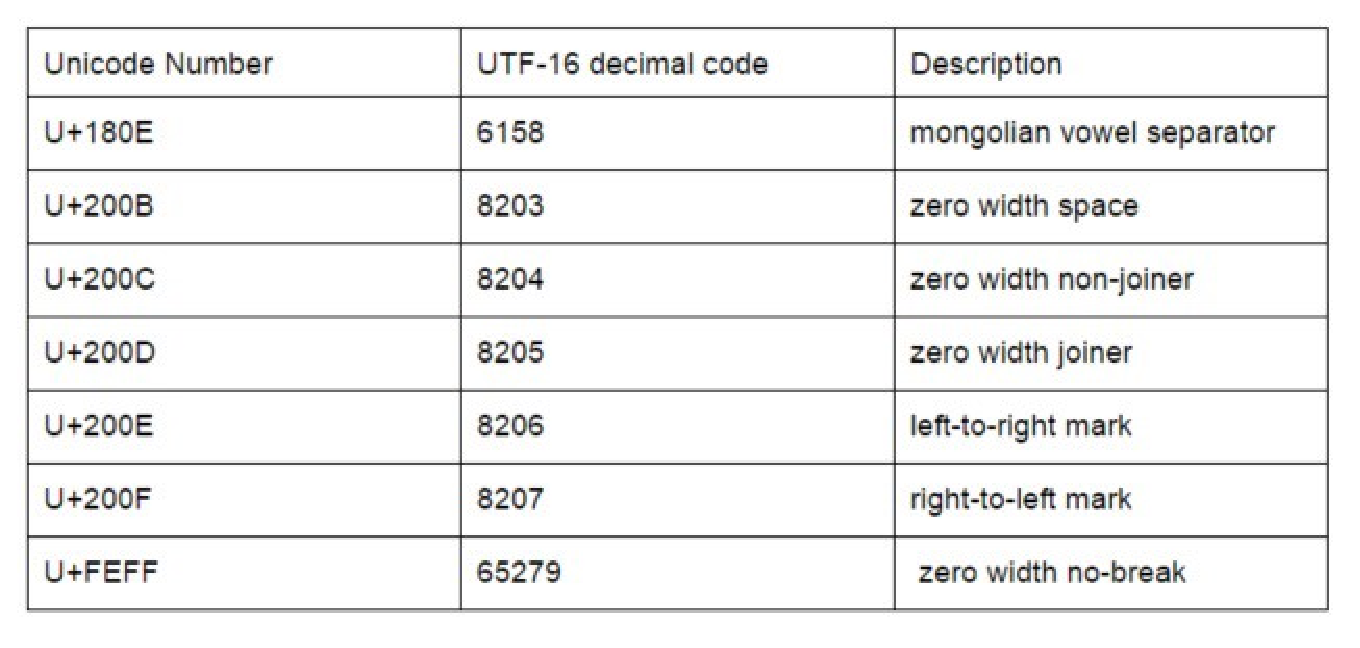
\includegraphics[width=1\textwidth]{img/zw-characters.eps}
\newline
Voici un exemple avec les caractères zero width space (ZWSP) et zero width non-joiner (ZWNJ) :
\newline
donnée : 'h'
\newline
valeur binaire : 01101000
\newline
Si l'on considère le caractère ZWSP comme valant 0 et ZWNJ comme valant 1 :
\begin{center}
\begin{tabular}{c c}
	0 & ZWSP \\
	1 & ZWNJ \\
	1 & ZWNJ \\
	0 & ZWSP \\
	1 & ZWNJ \\
	0 & ZWSP \\
	0 & ZWSP \\
	0 & ZWSP
\end{tabular}
\end{center}
On ajoute donc les caractères ZWSP ZWNJ ZWNJ ZWSP ZWNJ ZWSP ZWSP ZWSP à la fin du fichier, ceux-ci représentant les bits de la données insérée et n'étant pas vu par l'humain.
\subsubsection{Décodage}
Pour le décodage, il suffit de lire les zero width characters présents dan sle fichier et les convertir un par un en bits que l'on regroupe en octets pour pouvoir les convertirs en unicode.
